%!TEX root = ../dokumentation.tex
\chapter{Praxis Kapitel}
\section{Aufbau/Entwurf}
%TODO
\section{SDR Sharp}
SDR Sharp ist eine kostenlose Software von AIRSPY dir ausschließlich für Windows erhältlich ist. Mit dieser Anwendung kann man die empfangenen Rohdaten von USB Geräten auslesen, jedoch kann sie nur mit externer Hardware betrieben werden.  
%TODO Bild von SDR# hinzufügen
\section{GNU Radio}
GNU  Radio  ist  ein  freies  Open  Source  Entwicklerwerkzeug  zur  Implementierung von Software Defined Radio (SDR) mittels Signalverarbeitungsblöcken. Es kann mit externer Funkhardware oder als Simulation ohne Hardware genutzt werden. GNU Radio ist im Hobbybereich weit verbreitet, wird aber auch in der Wissenschaft und im kommerziellen Bereich genutzt. GNU Radio Programme kann zusätzlich  durch selbst programmierte Ergänzungsblöcke optimiert werden. Welche hauptsächlich in der Programmiersprache Python geschrieben, wobei echtzeitkritische Signalverarbeitungen auch in C++ implementiert werden kann.
%TODO Bild von GNU Radio hinzufügen
\subsection{Funktionsweise}
GNU Radio verarbeitet den Datenstrom, der vom Empfänger kommt, und bereitet Daten vor, um diese zu senden. Dabei ist die gesamte Datenverarbeitung in Blöcke eingeteilt,  die  beliebig  zusammengestellt  werden können. GNU Radio liefert eine Vielzahl von Filtern, Kanal-Codes, Synchronisationselementen, Equalizern, Demodulatoren, und vieles mehr. Diese  Blöcke  stellen  die  Hardwarekomponenten  klassischer  Funkhardware  dar. Falls nötig können auch selbst Blöcke hinzugefügt werden. Dabei sollte darauf geachtet werden, dass ein Block genau eine Aufgabe erledigt, damit er so vielseitig wie möglich eingesetzt werden kann. GNU Radio bietet die Möglichkeit, diese Blöcke miteinander zu verbinden und regelt dadurch den Datenfluss dazwischen. Für die digitale Verarbeitung von Daten kommen in GNU Radio verschiedene Datentypen zum Einsatz: Der Datenstrom des Empfängers besteht in den meisten Fällen aus komplexen Zahlen, also einem Datentyp, bei dem jedes Datum aus zwei Float-Werten, dem Imaginärteil und dem Realteil, besteht. Zwischen Blöcken können jedoch beliebige Datentypen zum Einsatz kommen, üblicherweise Short, Byte, Integer und Float. Der Datentyp am Eingang und Ausgang eines Blockes muss dabei nicht gleich sein.
Um mit GNU Radio eine SDR-Anwendung zu bauen, muss man Blöcke, die die einzelnen Funktionseinheiten darstellen, miteinander zu einem Graphen kombinieren. Sollte ein benötigter Block nicht verfügbar sein, kann man diesen mittels einem Tool selbst hinzufügen. Beim Starten des Graphen ruft GNU Radio nun jeden Block nacheinander auf und stellt sicher, dass Daten von einem Block zum Nächsten weitergereicht werden. Ergebnisse  können  durch  Graphical  User  Interface  (GUI)-Blöcke dargestellt werden. Diese nutzen die freien und plattformübergreifenden GUI-Toolkits.
\section{Hardware}
\subsection{Antenne}
Eine Antenne die aus der Aufgabenstellung hervorgeht, muss dementsprechend auch den Frequenzbereich der Dezimeterwelle abdeckt. Zu erst war die Überlegung eine mobile Antenne zu benutzen, somit könnte man die Analysefunktion des Gerätes auch unterwegs nutzen. Aus Gründen wie Flexibilität und Mobilität entschieden wir uns jedoch dagegen. Eine mobile Antenne, die den Frequenzbereich der Dezimeterwelle abdecken, würde relativ groß und ziemlich teuer sein. Deshalb haben wir uns auf eine stationäre Antenne geeinigt, da diese preislich als auch dem Verwendungszweck dennoch am Nähsten kommt. Wir haben uns für die  Sirio SD 3000N entschieden, ihr preis liegt bei 90 Euro und deckt den kompletten Frquenzbereich der Dezimeterwelle ab.\newline

\begin{figure}[H]
	\centering
	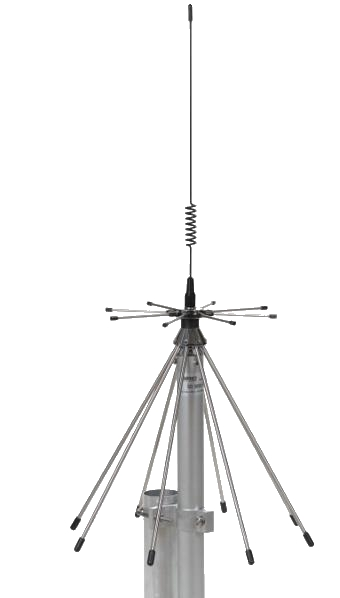
\includegraphics[width=0.3\textwidth]{SirioSD3000N.png}
	\caption[Sirio SD 3000N stationäre Funkantenne]{Sirio SD 3000N stationäre Funkantenne. Quelle: \cite{Funktechnik:2018}} 
	\label{Sirio SD 3000N Antenne}
\end{figure}

Auf Grund analytischen Zwecken haben werden zwei Antennen für die Aufgabe erworben, somit können wir an zwei unterschiedlichen Standorten eine Analyse der Metainformationen betrachten.
Präsentation vom Hochfrequenztechnik aus Mechtronik siehe WhatsApp

\subsection{SDR-Gerät}
Ein Software Defined Radio Gerät, das man experimentell betreiben kann, reicht von mehreren tausend Euro teuren Entwicklergeräten bis zu kostenlosen Geräten, da selbst mittels einem Mikrofoneingang der Soundkarte am Computers, derartige Signale empfangen werden können. Die Geräte unterscheiden sich hauptsächlich im Frequenzbereich, der maximalen Bandbreite und der Abtastrate. Beim Computer kommen häufig Universal Serial Bus (USB), Ethernet als Schnittstelle zum  Einsatz.
Da theoretische nur Signale empfangen werden sollen, würde ein DVB-T-Stick eine günstige Option darstellen. Mithilfe eines veränderten Treibers könnte der Stick mit GNU Radio genutzt werden, jedoch deckt sich der Frequenzbereich des Gerätes nicht, mit dem innerhalb der Aufgabenstellung der Dezimeterwelle.
Das SDR-Gerät muss in Kombination mit der Funkantenne den kompletten Funkbereich der Dezimeterwelle erstrecken, um die Metainformationen in diesem Bereich zu analysieren. Aus diesem Grund kann ein solchen Gerät für diese Arbeit nicht verwendet werden.
Eine mögliche Lösung ist das HackRF One Board. Die HackRF One Platine ist ein flexibles Testmodul für die Funkmesstechnik, das wie ein Software Defined Radio (SDR) arbeitet. Sie ist ein Open Source Hardware Transceiver, der hauptsächlich zu eigenen Versuchen und Messungen für SDRs eignet, außerdem ist dieses Gerät für die HF-Technik und messtechnischen Versuchsaufbauten im Amateurfunk vergleichsweise geringen Preises von rund 300 Euro sehr beliebt.
Der Hack RF One deckt einen weiten Frequenzbereich von 1 bis 6000 MHz (6 GHz) ab, und erfasst damit sehr viele Frequenzbänder für kommerzielle, experimentelle und Amateurfunk-Anwendungen. Die Hardware bietet eine maximale Abtastrate des Signales von 20MS/s, dadurch werden Messungen und Experimente auch mit breitbandigen Signalen wie DECT, WFM oder WLAN möglich, jedoch nur halbduplex. Der AD-Wandler arbeitet mit 8 Bit Datenbreite und erreicht somit einen theoretischen Dynamikbereich von 48dB. Die digitalisierten I/Q Daten werden auf einem nachgeschalteten CPLD weiterverarbeitet und über den integrierten ARM-Prozessor per USB ausgegeben. Die gesamte Schaltung des HackRF Boards ist sehr stromsparend ausgelegt, sie wird komplett über USB versorgt. Die Platine hat eine Mikro-B USB Buchse. Abschließend lässt sich sagen, dass die oben genannten Gründe für eine Nutzung dieses Gerätes sprechen.\cite{wimo:2018}
\begin{figure}[H]
	\centering
	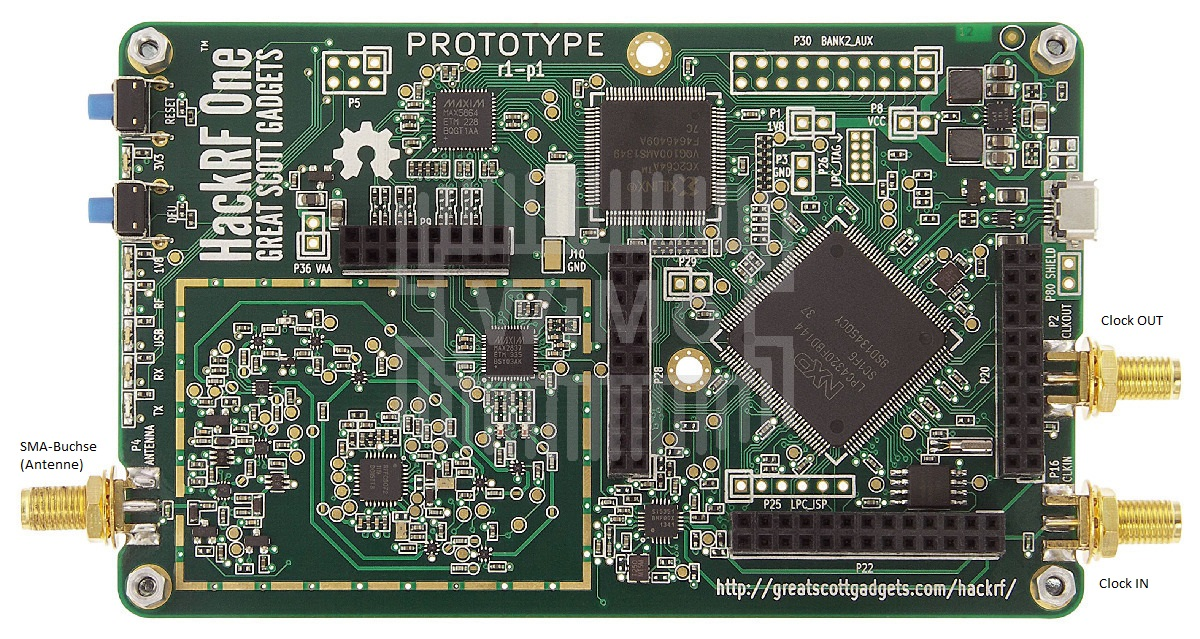
\includegraphics[width=0.75\textwidth]{HackRFOne.png}
	\caption[Hack RF ONE Platine]{Hack RF ONE Platine. Quelle: \cite{HackRFOne:2018}} 
	\label{HackRFOne}
\end{figure}
